\section{Testing in Azure CI/CD [Mohammed Mehedi Hasan]}

Testing is one of the most important part in CI/CD automation. The test execution helps the automation process more fail-safe and bug free. In Azure, we are using \textbf{Azure Test Plans} is used for test execution and report generation. For every CI pipeline run, test execution is an integral process. Without passing all the test cases the CI pipeline will not move froward and deemed as failed execution. As a consequences, CD pipeline will also not be executed. By this mechanism we are making sure that there are no bugs in the application.

In our testing strategy, we are executing all the \textbf{Unit} and \textbf{Integration} test to make sure the new changes do not break the existing running application and infrastructure as well. The test cases are executed when the gradle build task is run CI pipeline. Upon success or failure of the test execution azure test plans generate a report and saved it. One can download the report from test runs and analyse it as required. The test result is always CI run specifics. For every run a new test report is generated.In figure \ref{fig:test_run_dashboard}, the summary of each test execution is displayed.

\begin{figure}[h]
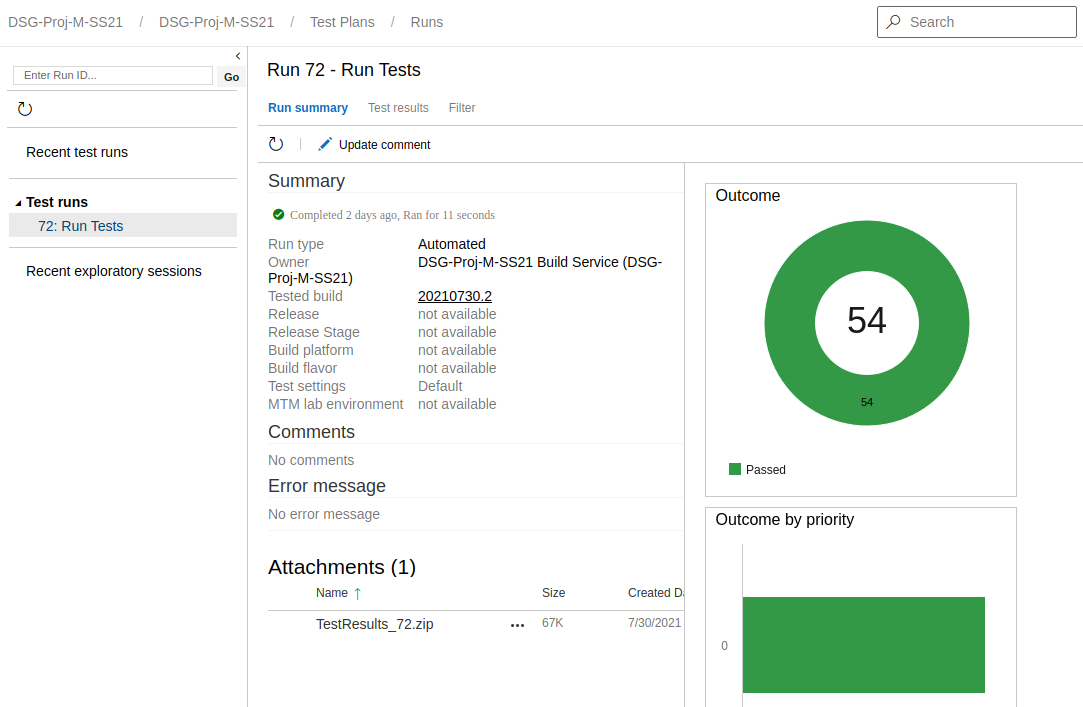
\includegraphics[scale=0.40]{images/mehedi/testReportDashboard.png}
\centering
\caption{Test Run Dashboard}
\label{fig:test_run_dashboard}
\end{figure}

Additionally, one can see the test execution summary and overall analysis of specific test run in azure test plans. The every test execution result for every test cases of every run can also be found out in test plans as well. How many times it toke to execute the test cases, the result of the execution and in case of failure the reason is shown as well. Figure \ref{fig:specific_test_case} shows how one can see individual test case execution summary.

\begin{figure}[h]
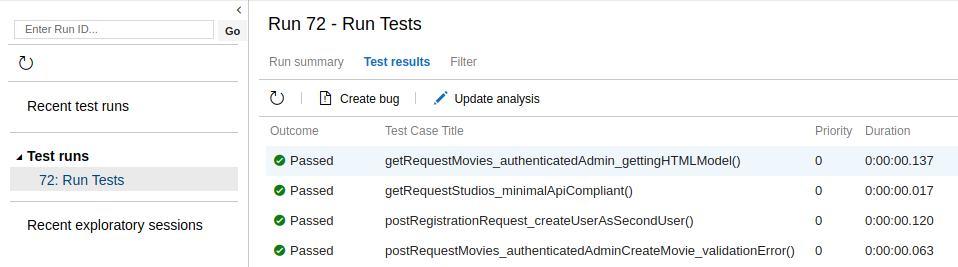
\includegraphics[scale=0.40]{images/mehedi/specificTestCases.png}
\centering
\caption{Individual Test Case Analysis}
\label{fig:specific_test_case}
\end{figure}
